%----------------------------------------------------------------------%
% 軌道解析コード「Tacode」version 2: 理論・検証・実証
% Yusuke Takahashi, Hokkaido University
% 日本語版（正は英語版 tacode_v2_en.tex）
%----------------------------------------------------------------------%
\documentclass[11pt,a4paper,dvipdfmx]{jsarticle}

\usepackage[dvipdfmx]{graphicx}
\usepackage[dvipdfmx]{color}
\usepackage{amsmath, amsfonts, amssymb}
\usepackage{array}
\usepackage{url}
\usepackage{fancyhdr}
\usepackage{listings}
\usepackage[margin=25mm]{geometry}

\graphicspath{ {./figure/} }

\pagestyle{fancy}
\setlength{\headheight}{16pt}
\fancyhf{}
\rhead{\thepage}
\lhead{Tacode version 2: 理論・検証・実証}

\lstset{%
  basicstyle={\small\ttfamily},
  backgroundcolor={\color[gray]{.95}},
  frame=single,
  breaklines=true,
  columns=fullflexible,
  xleftmargin=2em,
  xrightmargin=0em,
  lineskip=-0.3ex
}

\newcommand{\bx}{{\boldsymbol x}}
\newcommand{\bv}{{\boldsymbol v}}
\newcommand{\bF}{{\boldsymbol F}}
\newcommand{\bM}{{\boldsymbol M}}
\newcommand{\bI}{{\boldsymbol I}}
\newcommand{\bq}{{\boldsymbol q}}
\newcommand{\bOm}{{\boldsymbol \Omega}}
\newcommand{\bom}{{\boldsymbol \omega}}
\newcommand{\bC}{{\boldsymbol C}}
\newcommand{\bR}{{\boldsymbol R}}

%----------------------------------------------------------------------%
\begin{document}

\begin{center}
{\LARGE \bf 軌道解析コード「Tacode」version 2 \\[3mm]
理論・検証・実証}
\end{center}

\begin{center}
{\normalsize
  高橋 裕介\footnote{E-mail: ytakahashi@eng.hokudai.ac.jp} \\
  {\itshape 北海道大学、〒060-8628 北海道札幌市北区北 13 条西 8 丁目}
}
\end{center}

\vspace{3mm}
\noindent
{\small
{\bf 概要}\quad
Tacode は、惑星中心・惑星固定の回転座標系で質点の運動方程式を、version 2.3 以降は
剛体の運動方程式を積分する軌道解析コードである。本稿の version 1 では 3 自由度の
定式化とコードの操作を述べた。本稿では version 2 を述べる。すなわち 6 自由度への
拡張、揚力とバンク角、風、絶対時刻、およびそれらとともに入れた数値的な安全装置で
ある。そのうえで、コードが正しいことを示すために何をしたかを報告する。検証
(verification) は、厳密解・物理的な恒等式・変異テストに基づく 488 件の自動テストに
よって行い、時間積分の実測収束次数を測った。実証 (validation) は 3 つの飛行、
Apollo 4（1967 年）、Apollo 10（1969 年）、Project Fire flight II（1965 年）に対して
行った。最後の 1 つは詳しく扱う。姿勢ソルバーを実測データで叩ける飛行として見つかった
唯一のものであり、また「何が確かめられて何が確かめられないか」を決めるまでの筋道
そのものが結果の一部だからである。
}

%----------------------------------------------------------------------
\section*{記号}
\begin{tabbing}
\hspace{7.0em}\= \hspace{1.5em} \= \hspace{10cm} \kill
	$a_e$      \> = \> 赤道半径（長半径）, m \\
	$C_D, C_L$ \> = \> 抗力係数・揚力係数 \\
	$C_{F}, C_{M}$ \> = \> 機体軸の力係数・モーメント係数 \\
	$C_{lp}, C_{mq}, C_{nr}$ \> = \> 動的減衰微係数, 1/rad \\
	$\bC_{b/e}$ \> = \> ECEF から機体軸への変換行列 \\
	$d$        \> = \> 基準直径, m \\
	$e$        \> = \> 第 1 離心率 \\
	$f$        \> = \> 扁平率 \\
	$\bF$      \> = \> 力ベクトル, N \\
	$G$        \> = \> 万有引力定数, m$^3$/kg$\cdot$s$^2$ \\
	$H$        \> = \> 測地座標系の高度, m \\
	$\bI$      \> = \> 重心まわりの慣性テンソル, kg m$^2$ \\
	$J$        \> = \> 力学的形状係数 \\
	$Kn$       \> = \> Knudsen 数 \\
	$L$        \> = \> 基準長, m \\
	$m$        \> = \> 機体質量, kg \\
	$M$        \> = \> 惑星質量, kg \\
	$\bM$      \> = \> モーメントベクトル, N m \\
	$p, q, r$  \> = \> ECEF に対する角速度の機体軸成分, rad/s \\
	$q_{\infty}$ \> = \> 動圧, N/m$^2$ \\
	$\bq$      \> = \> 姿勢クォータニオン（スカラー先頭） \\
	$r$        \> = \> 極座標系の動径, m \\
	$\bR_x$    \> = \> 機体 $x$ 軸まわりの回転行列 \\
	$S$        \> = \> 基準面積, m$^2$ \\
	$t$        \> = \> 時刻, s \\
	$U$        \> = \> 重力ポテンシャル, m$^2$/s$^2$ \\
	$\bv$      \> = \> ECEF 系の速度ベクトル, m/s \\
	$\bx$      \> = \> ECEF 系の位置ベクトル, m \\
	$\alpha$   \> = \> 極座標系の経度, rad（迎角にも用いる） \\
	$\alpha_t$ \> = \> 全迎角, rad \\
	$\beta$    \> = \> 極座標系の緯度, rad（横滑り角にも用いる） \\
	$\eta$     \> = \> 全迎角, deg（Fire の報告書の記法） \\
	$\lambda$  \> = \> 測地座標系の経度, rad \\
	$\rho$     \> = \> 大気密度, kg/m$^3$ \\
	$\sigma$   \> = \> バンク角, rad \\
	$\phi$     \> = \> 測地座標系の緯度, rad \\
	$\varphi_a$ \> = \> 空力ロール角, rad \\
	$\bom$     \> = \> 惑星の角速度ベクトル, rad/s \\
	$\bOm$     \> = \> 慣性系に対する機体の角速度, rad/s \\
	$\bOm_{\rm rel}$ \> = \> ECEF 系に対する機体の角速度, rad/s \\
\end{tabbing}

%----------------------------------------------------------------------
\section{はじめに}

宇宙機の軌道は、他のすべての分野が設計対象とする環境を決める。動圧、熱流束、軌道上の
寿命、着地点の散らばりがそれである。したがって軌道解析ツールは開発の早い段階から
繰り返し使われるものであり、扱いが簡単で、他のツールと繋ぎやすく、そして
「何をモデル化していて何をしていないか」について正直であるほど価値が高い。

本稿の前身で述べた Tacode version 1 は、惑星の回転系における質点の並進 3 自由度を
積分するものであった。重力は球面調和関数で展開し、回転系のコリオリ力と遠心力を持ち、
抗力はテーブル化した大気から読む。弾道的な再突入や打ち上げにはこれで足り、実際に
そのように使われてきた。

しかし、その後に出てきた 3 つのことにはこれでは足りない。第一に、鈍頭の再突入
カプセルは揚力を持って飛び、その揚力の向き（バンク角）こそ誘導系が指令する量である。
これが無いと、揚力を持つ再突入の計算軌道は数パーセントではなく数十 km ずれる。
第二に、無制御の機体の姿勢は振動し、その周期と振幅こそスピン安定プローブの設計量で
あるが、質点はそれについて何も言えない。第三に、対流圏まで降りる再突入は風下へ流され、
これは共回転する大気では表せない。

version 2 はこの 3 つをすべて足し、あわせて日付に依るモデルを駆動するための絶対時刻と、
数値的な安全装置を入れた。何がいつ入ったかを表 \ref{version_history} に示す。

\begin{table}[h]
\caption{Tacode 2 の各版が足したもの。\textbf{新しいモデルはすべて既定で無効}であり、
無効なら出力はバイト単位で変わらない。これは回帰テストで強制している。}
\label{version_history}
\begin{center}
\small
\begin{tabular}{l|l}
\hline \hline
版 & 追加されたもの \\
\hline
2.0 -- 2.2 & version 1 の定式化の Python 実装 \\
2.3.0 & 6 自由度: 姿勢クォータニオン、Euler 方程式、$\alpha_t$ を軸とする空力テーブル \\
2.3.1 & 空力データベースが軸対称でないときの警告 \\
2.4.0 & 風、および絶対時刻（エポック） \\
2.5.0 & 3 自由度の揚力とバンク角、発散の検知、 \\
      & モンテカルロの失敗検知と乱数種、飛行実測との突き合わせ \\
\hline \hline
\end{tabular}
\end{center}
\end{table}

本稿の後半は機能ではなく正しさについてである。軌道解析コードは書くのは易しく、信じる
のが難しい。係数が広い範囲で間違っていても出力はもっともらしく見え、普段は小さい項の
符号の誤りは、それが大きくなる場合が来るまで見えない。第 \ref{verification} 章で
検証の方針を、第 \ref{validation} 章で 3 つの実飛行との突き合わせを述べる。

%----------------------------------------------------------------------
\section{数理モデル}

\subsection{状態ベクトルと自由度}

Tacode は図 \ref{cartesian_coordinate} の地球中心・地球固定（ECEF）回転系で状態
ベクトルを進める。3 自由度では状態は質点の位置と速度である。
\texttt{attitude.flag\_attitude: True} とすると剛体の姿勢クォータニオンと角速度が加わる。
%
\begin{align}
	{\boldsymbol y} = \left[ \bx, \; \dot{\bx} \right] \quad \textrm{(3 自由度)} ,
	\qquad
	{\boldsymbol y} = \left[ \bx, \; \dot{\bx}, \; \bq, \; \bOm \right] \quad \textrm{(6 自由度)} .
\end{align}
%
どちらも同じ積分器・同じ時間刻みで進める。並進と回転は双方向に結合している。モーメントが
機体を回し、空力は姿勢に従う。以下の力のうち姿勢に依存するのは空力だけなので、姿勢を
切れば並進の組は version 1 の 3 自由度方程式に\emph{厳密に}帰着する。

\begin{figure}[h]
\begin{center}
	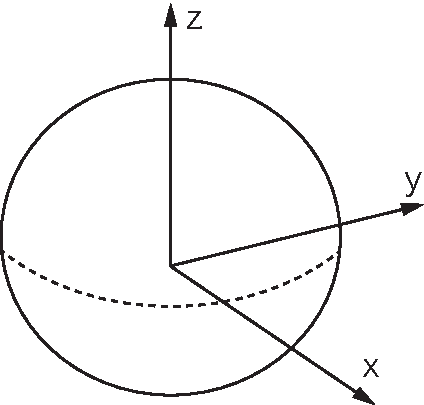
\includegraphics[width=0.30\linewidth]{cartesian_coordinate}
\end{center}
\caption{直交（ECEF）座標系。}
\label{cartesian_coordinate}
\end{figure}

\subsection{並進運動}

非慣性系である ECEF 系での質点の運動方程式は
%
\begin{align}
	m \frac { \partial^{2} \bx }{ \partial t^{2} } =
	\bF_{\rm grav}
	- 2 m \bom \times \frac { \partial \bx }{ \partial t }
	- m \bom \times \left( \bom \times \bx \right)
	+ \bF_{\rm aero} ,
	\label{law_momentum}
\end{align}
%
である。$t$ は時刻、$\bx$ と $m$ は位置ベクトルと質量、$\bom$ は座標系の角速度で、
地球では $\bom = (0, 0, 7.292115\times10^{-5})$ rad/s である。右辺第 2 項と第 3 項は
座標系が回転するために現れるコリオリ力と遠心力で、赤道では遠心力は重力の約 1 \% である。

\subsection{回転運動}

重心まわりの剛体の回転は、慣性テンソルが一定になる機体軸で書いた Euler 方程式に従う。
%
\begin{align}
	\bI \frac{ \partial \bOm }{ \partial t }
	+ \bOm \times \left( \bI \bOm \right)
	= \bM_{\rm aero} + \bM_{\rm damp} + \bM_{\rm grav} .
	\label{law_euler}
\end{align}
%
ここで $\bOm$ は\emph{慣性系に対する}角速度を機体軸成分で表したもので、右辺の 3 項は
空力・動的減衰・重力傾斜のモーメントであり、それぞれ個別に切ることができる。

\subsection{座標系}

4 つの座標系を使う。取り違えると効くので、規約をまとめて挙げる。

\begin{itemize}
\item \textbf{ECEF 直交系}（図 \ref{cartesian_coordinate}）が方程式を積分する系である。
$x$ 軸が経度 $0$、$y$ 軸が経度 $90^\circ$、$z$ 軸が極を通る。
\item \textbf{測地座標系}（図 \ref{geodetic_coordinate} 左）は WGS84 回転楕円体上の
緯度 $\phi$・経度 $\lambda$・高度 $H$ である。初期位置の与え方と出力の書き方がこれである。
$N = a_e / \sqrt{1 - e^2 \sin^2\phi}$、$e^2 = f(2-f)$ として
\begin{align}
	X = (N+H) \cos\phi \cos\lambda , \quad
	Y = (N+H) \cos\phi \sin\lambda , \quad
	Z = \left[ N(1-e^2) + H \right] \sin\phi ,
\end{align}
地球では $a_e = 6.3781370 \times 10^6$ m、$f = 1/298.257223563$ である。逆変換は
Bowring 型の閉じた反復で解く。
\item \textbf{地心極座標系}（図 \ref{geodetic_coordinate} 右）は動径 $r$・経度 $\alpha$・
緯度 $\beta$ で、重力を評価する系である。
\item \textbf{ローカル水平系}は地心の北東下（NED）系、\textbf{機体軸}は
[前方, 右, 下] である。Tacode が読み書きするオイラー角は、ローカル水平系から機体軸への
3-2-1（ヨー・ピッチ・ロール）で、ヨーは北から東回りに測る。
\end{itemize}

\begin{figure}[h]
\begin{center}
	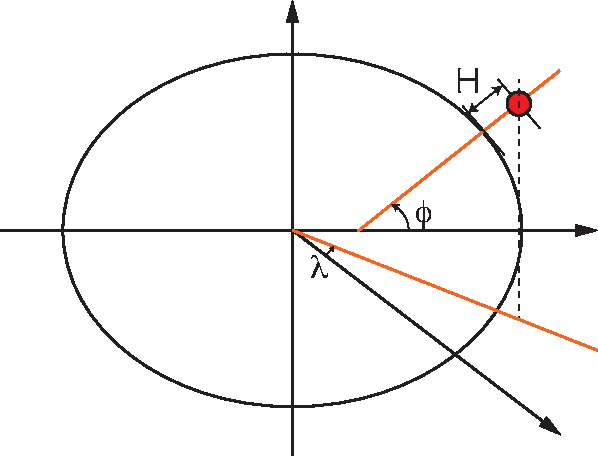
\includegraphics[width=0.28\linewidth]{geodetic_coordinate}
	\hspace{12mm}
	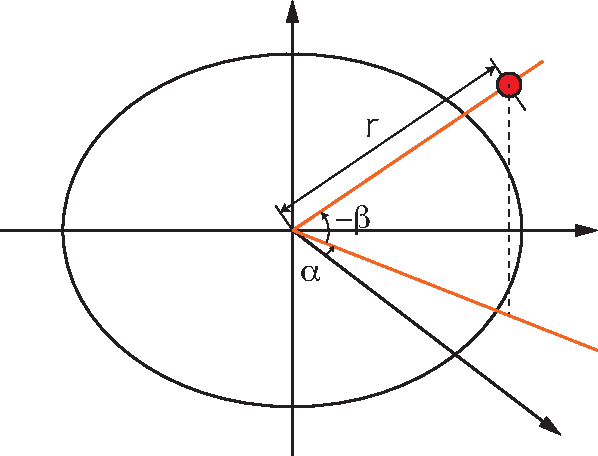
\includegraphics[width=0.28\linewidth]{polar_coordinate}
\end{center}
\caption{測地座標系（左）と地心極座標系（右）。}
\label{geodetic_coordinate}
\end{figure}

\textbf{ひとつだけ繰り返しておきたい規約がある。}初期位置は\emph{測地}系だが、初期速度は
\emph{地心}ローカル水平系 [東, 北, 上] で与え、風も同じである。この 2 つの鉛直は最大
$0.19^\circ$ 違う。コード自体は自己整合している（出力も地心である）が、外部から
持ってきた状態ベクトルは変換しなければならず、第 \ref{validation} 章の実証ケースは
それぞれその変換スクリプトを自前で持っている。

\subsection{重力}

惑星は回転楕円体なので、ポテンシャルは極座標系で球面調和関数に展開する
\cite{Wagner1966,Liu2019}。
%
\begin{align}
	U = - \frac{G M}{r}
	\left[ 1
	- \left( \frac{a_{e}}{r} \right)^2 J_{20} \frac{ 3 \sin^2 \beta - 1}{2}
	- \left( \frac{a_{e}}{r} \right)^2 J_{22} \, 3 \cos^2 \beta \cos 2 \left( \alpha + \alpha_{22} \right) \right.
	\nonumber \\
	\left.
	- \left( \frac{a_{e}}{r} \right)^3 J_{30} \frac{ 5 \sin^3 \beta - 3 \sin \beta}{2}
	- \left( \frac{a_{e}}{r} \right)^4 J_{40} \frac{1}{8} \left( 35 \sin^4 \beta - 30 \sin^2 \beta + 3 \right) \right] .
\end{align}
%
これを極座標成分で微分したものが $\bF_{\rm grav}$ であり、直交系に変換して使う。
各項が何を表しているかを図 \ref{potential_schematic} に示す。等ポテンシャル面が球から
ずれており、$J$ の各項がそのずれの 1 つのモードである。地球で使うパラメータを
表 \ref{J_parameters} に示す。これらは設定ファイルの項目なので、他の惑星は値を変えて
大気テーブルを用意すれば扱える。

\begin{figure}[h]
\begin{center}
	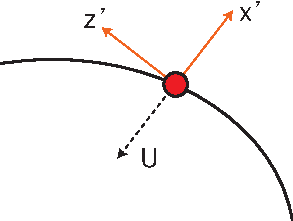
\includegraphics[width=0.30\linewidth]{potential_schematic}
\end{center}
\caption{$J$ 項の展開が記述する、回転する回転楕円体の等ポテンシャル面。}
\label{potential_schematic}
\end{figure}

\begin{table}[h]
\caption{地球に対する力学的形状係数（\texttt{planet.potential\_factor}）。}
\label{J_parameters}
\begin{center}
\begin{tabular}{l|r|l|r}
\hline \hline
パラメータ & 値 & パラメータ & 値 \\
\hline
$J_{20}$ & $1.082629 \times 10^{-3}$   & $J_{40}$ & $-1.62336 \times 10^{-6}$ \\
$J_{22}$ & $-1.81222 \times 10^{-6}$   & $\alpha_{22}$ & $-14.545$ deg \\
$J_{30}$ & $-2.5356 \times 10^{-6}$    & $GM$ & $3.98600 \times 10^{14}$ m$^3$/s$^2$ \\
\hline \hline
\end{tabular}
\end{center}
\end{table}

\subsection{空力}

動圧は $q_{\infty} = \frac{1}{2} \rho \left| \bv_{\rm air} \right|^2$ である。
$\bv_{\rm air}$ は対気速度で、風を切っていれば大気は惑星と共回転するので
$\bv_{\rm air} = \bv$ になる。

\paragraph{3 自由度。}
姿勢が分からないので、力は運動方向の抗力になる。
%
\begin{align}
	\bF_{\rm drag} = - q_{\infty} C_D S \frac{ \bv_{\rm air} }{\left| \bv_{\rm air} \right|} ,
\end{align}
%
これに、速度に直交する揚力を足すことができる。揚力の面内での向きはバンク角 $\sigma$ が
決める（図 \ref{body_axes} 右）。
%
\begin{align}
	\bF_{\rm lift} = q_{\infty} C_L S \left( \cos\sigma \, \hat{\boldsymbol n}_u + \sin\sigma \, \hat{\boldsymbol n}_r \right) ,
	\quad
	\hat{\boldsymbol n}_u = \frac{ \hat{\boldsymbol u} - ( \hat{\boldsymbol u} \cdot \hat{\bv} ) \hat{\bv} }{ \left| \cdot \right| } ,
	\quad
	\hat{\boldsymbol n}_r = \hat{\bv} \times \hat{\boldsymbol n}_u ,
	\label{lift}
\end{align}
%
ここで $\hat{\boldsymbol u} = \bx / |\bx|$ は地心の鉛直である。したがって $\sigma = 0$ で
揚力は上向き、$\sigma = 180^\circ$ で下向きになる。\textbf{Tacode は誘導則を持たない。}
バンク角は定数か、時刻に対する表として与える。後者が\emph{実測の}ロール履歴を飛ばす
方法である。表は Runge--Kutta の各段が自分の時刻で引く。$C_L = 0$ なら揚力は評価すら
されないので、これを書かない設定は version 1 の結果をビット単位で再現する。

\paragraph{6 自由度。}
力は全迎角と Knudsen 数を軸とする機体軸のテーブルから読む。対気速度の機体軸成分を
$[u, v, w] = \bC_{b/e} \bv_{\rm air}$ と書くと（図 \ref{body_axes} 左）、
%
\begin{align}
	\alpha_t = \arccos \frac{u}{\left| \bv_{\rm air} \right|} , \qquad
	\varphi_a = \arctan \frac{v}{w} ,
\end{align}
%
であり、$\alpha_t$ は機体 $x$ 軸と速度のなす角、$\varphi_a$ は係数を表にした面と、
実際に横流れがある面とのなす角である。テーブルを $\alpha_t$ で引き、機体 $x$ 軸まわりに
その面へ回す。
%
\begin{align}
	\bF_{\rm aero} = - q_{\infty} S \, \bC_{F} ,
	\qquad
	\bC_{F} = \bR_{x} \left( \varphi_a \right)
	\begin{bmatrix} C_{Fx} \\ C_{Fy} \\ C_{Fz} \end{bmatrix} \left( \alpha_t, Kn \right) .
	\label{force_6dof}
\end{align}
%
これは回転体に対しては\emph{厳密}である。$\alpha_t$ だけを軸とする表が記述しているのは
まさに回転体だからである。軸対称でない表は読み込み時に報告し、黙って使うことはしない。
符号は、迎角 0 で $\bC_F = [C_D, 0, 0]$ となり式 (\ref{force_6dof}) が 3 自由度の抗力に
一致するように選んである。したがって両者は $\alpha_t = 0$ で最後のビットまで一致し、
テストがそれを検査している。

\begin{figure}[h]
\begin{center}
	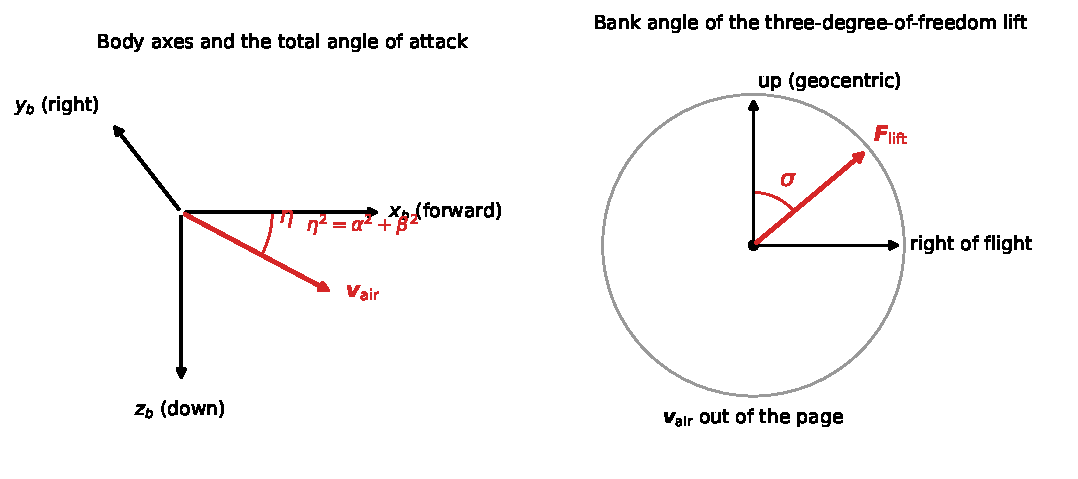
\includegraphics[width=0.92\linewidth]{body_axes}
\end{center}
\caption{左: 機体軸と全迎角 $\eta = \alpha_t$。右: 対気速度に直交する面内での
3 自由度の揚力とバンク角 $\sigma$。}
\label{body_axes}
\end{figure}

\subsection{空力モーメント・減衰・重力傾斜}

モーメント係数は同じテーブルの同じ $\alpha_t$ から読み、同じ $\bR_x(\varphi_a)$ で回す。
これは固有回転なので、モーメントの擬ベクトルは力ベクトルと厳密に同じように変換される。
そのうえで、テーブルの基準点から重心へ移す。
%
\begin{align}
	\bM_{\rm aero} = q_{\infty} S L \, \bC_{M}
	+ \left( {\boldsymbol r}_{\rm ref} - {\boldsymbol r}_{\rm cg} \right) \times \bF_{\rm aero} ,
	\qquad
	\bC_{M} = \bR_{x} \left( \varphi_a \right)
	\begin{bmatrix} C_{Mx} \\ C_{My} \\ C_{Mz} \end{bmatrix} \left( \alpha_t, Kn \right) .
	\label{moment_aero}
\end{align}
%
機体軸を [前方, 右, 下] に取ると $C_{My}$ が正で機首上げなので、静安定な機体は正の
迎角で $C_{My} < 0$ になる。

テーブルが与えるのは静的係数、すなわち姿勢を固定した機体に働くモーメントである。
回転している機体はその回転に逆らうモーメントも受ける。
%
\begin{align}
	\bM_{\rm damp} = q_{\infty} S L \frac{L}{2 \left| \bv_{\rm air} \right|}
	\begin{bmatrix} C_{lp} \, p \\ C_{mq} \, q \\ C_{nr} \, r \end{bmatrix} .
	\label{moment_damp}
\end{align}
%
これが無いと、静安定な機体の振動は決して減衰しない。静的係数だけでは保存系だからである。
最後に、機体を横切る重力勾配の 1 次の効果は
%
\begin{align}
	\bM_{\rm grav} = \frac{3 G M}{r^3} \, \hat{\boldsymbol u} \times \left( \bI \hat{\boldsymbol u} \right) ,
	\qquad
	\hat{\boldsymbol u} = \bC_{b/e} \frac{ \bx }{ \left| \bx \right| } ,
\end{align}
%
で、慣性テンソルが等方なとき、および主軸が $\hat{\boldsymbol u}$ に揃っているときに
消える。低軌道の小型機では $10^{-6}$ N m の桁で、再突入中は空力モーメントに比べて
無視できるが、真空中では唯一残るモーメントである。

\subsection{姿勢のキネマティクスと、2 種類の角速度}

姿勢は ECEF から機体軸への変換を表すクォータニオン $\bq = [q_0, q_1, q_2, q_3]$
（スカラー先頭）が担う。オイラー角そのものを使わないのは特異点が無いからで、
再突入体がピッチ $90^\circ$ を通ると 3-2-1 のジンバルロックに当たる。その発展式は
%
\begin{align}
	\frac{ \partial \bq }{ \partial t } = \frac{1}{2} {\boldsymbol Q} \left( \bOm_{\rm rel} \right) \bq ,
	\qquad
	{\boldsymbol Q} = \begin{bmatrix}
	0 & -p & -q & -r \\
	p & 0 & r & -q \\
	q & -r & 0 & p \\
	r & q & -p & 0 \end{bmatrix} .
\end{align}
%
\textbf{角速度が 2 種類現れ、取り違えてはいけない。}Euler 方程式 (\ref{law_euler}) は
\emph{慣性系}に対する角速度 $\bOm$ で書かれているが、クォータニオンは回転する ECEF 系を
基準にしているので、
%
\begin{align}
	\bOm_{\rm rel} = \left[ p, q, r \right] = \bOm - \bC_{b/e} \bom
\end{align}
%
で発展する。惑星の自転を残すと姿勢が 0.0042 deg/s で漂流する。空力減衰
(\ref{moment_damp}) が見るのも同じ相対角速度である。大気が共回転しているからである。
積分される量は $\bOm$ だが、設定ファイルの入力と結果ファイルの出力はどちらも
$\bOm_{\rm rel}$ で、こちらのほうが人間には直観的なので、コードが境界で変換する。
クォータニオンは積分の各段で正規化する。

\subsection{風}

風は「大気が惑星と剛体的に共回転する」という仮定を緩めるだけである。
%
\begin{align}
	\bv_{\rm air} = \bv - \bv_{\rm wind} ({\rm ECEF}) .
\end{align}
%
\textbf{これを見るのは空力だけ}である。抗力、6 自由度の力とモーメント、動圧、空力角が
それにあたる。重力・コリオリ力・遠心力・角速度は触らない。風は並進の量であって系の
回転ではないからである。風は地心ローカル水平系 [東, 北, 上] で与える。初期速度と
同じ系であり、気象データの $u$/$v$ の測地系とは最大 $0.19^\circ$ 傾くが、コードが
規約を 2 つ持たないほうを選んだ。風を切っているときは引き算自体を通さないので、
結果は従来の定式化とビット単位で一致する。

\subsection{絶対時刻}

初期条件に絶対時刻を付けることができる。質点の定式化にこれは要らないが、時刻軸を持つ
風テーブルには必要であり、日付に依るモデルすべての土台になる。エポックは結果ファイルの
ヘッダに書く。出力形式がデータ行に文字列を持てないからである。閏秒は考慮せず、
ECEF--ECI 変換は現時点で無い。

%----------------------------------------------------------------------
\section{離散化モデル}

\subsection{時間積分}

式 (\ref{law_momentum}) の右辺を $\bF$、式 (\ref{law_euler}) を対応する角加速度と書けば、
系は 1 階の方程式の組であり、1 次精度の陽的 Euler 法
%
\begin{align}
	\bx^{n+1} = \bx^{n} + \bv^{n} \Delta t , \qquad
	\bv^{n+1} = \bv^{n} + \bF^{n} \Delta t ,
	\label{euler}
\end{align}
%
か、4 段 4 次 Runge--Kutta 法
%
\begin{align}
&	{\boldsymbol k}_1 = {\boldsymbol f} \left( t^n, {\boldsymbol y}^n \right) \Delta t , \qquad
	{\boldsymbol k}_2 = {\boldsymbol f} \left( t^n + \tfrac{1}{2}\Delta t, {\boldsymbol y}^n + \tfrac{1}{2}{\boldsymbol k}_1 \right) \Delta t , \nonumber \\
&	{\boldsymbol k}_3 = {\boldsymbol f} \left( t^n + \tfrac{1}{2}\Delta t, {\boldsymbol y}^n + \tfrac{1}{2}{\boldsymbol k}_2 \right) \Delta t , \qquad
	{\boldsymbol k}_4 = {\boldsymbol f} \left( t^n + \Delta t, {\boldsymbol y}^n + {\boldsymbol k}_3 \right) \Delta t , \\
&	{\boldsymbol y}^{n+1} = {\boldsymbol y}^{n} + \tfrac{1}{6} \left( {\boldsymbol k}_1 + 2 {\boldsymbol k}_2 + 2 {\boldsymbol k}_3 + {\boldsymbol k}_4 \right) \nonumber
\end{align}
%
で進める。姿勢も同じ段で進め、各段のあとにクォータニオンを正規化する。時間刻みは一定である。

間違えやすい点を 2 つ記録しておく。第一に、\textbf{風とバンク角の表は各段が自分の時刻で
引く}。段の係数は $[0, \frac{1}{2}, \frac{1}{2}, 1]$ であり、ステップの時刻で引くと
黙って次数が落ちる。第二に、\textbf{出力}に載る大気量は 1 段目、すなわち出力される位置で
評価した値である。4 段目の値を出すと 1 ステップぶんずれる。

\subsection{収束次数}

図 \ref{order_of_accuracy} は、第 \ref{fire2} 節の Project Fire II 再突入（73 $g$ の
減速を通る）で実測した収束次数である。固定した時刻の状態を、最も細かい刻みの計算と
比べている。細かいほうの 3 点で測った傾きは、3 自由度の位置で $4.3$、6 自由度の姿勢
クォータニオンで $3.9$ であり、どちらもスキームの 4 次である。

この図について 2 つ言っておきたい。粗いほうの端は 4 次の線から\emph{離れる}。その刻みでは
減速のピークや姿勢振動を解けていないからで、漸近域は仮定するものではなく探すものである。
また、テーブルの内挿が到達点を制限する。迎角のテーブルは $C^0$ でしかないので、迎角が
テーブルの節点をまたぐ場合の収束次数は 4 ではなく 2 から 3 の間になる。これはテストが
別に測っている。

\begin{figure}[h]
\begin{center}
	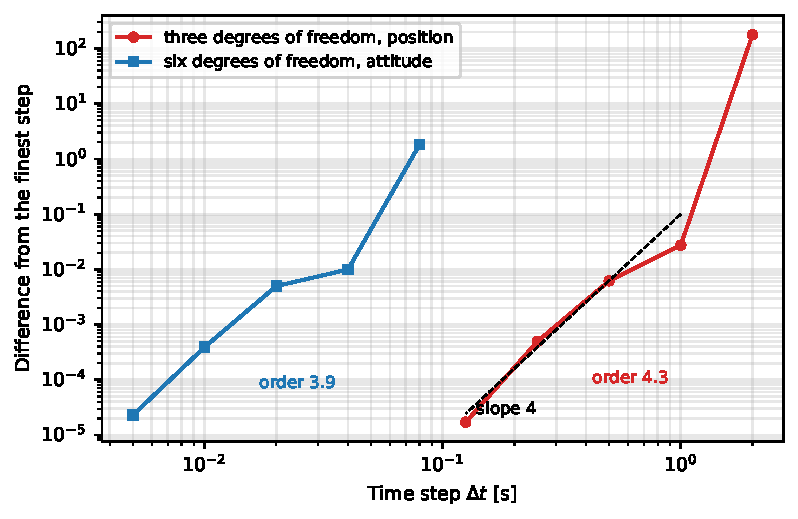
\includegraphics[width=0.62\linewidth]{order_of_accuracy}
\end{center}
\caption{Project Fire II 再突入で実測した収束次数。最も細かい刻みの計算との差を固定した
時刻で取った。破線は傾き 4。縦軸は 3 自由度では距離 [m]、6 自由度ではクォータニオンの
差のノルムである。}
\label{order_of_accuracy}
\end{figure}

\subsection{姿勢の時間刻み}

静安定な機体の振動周期
%
\begin{align}
	T = 2 \pi \sqrt{ \frac{I_{yy}}{ q_{\infty} S L \left| C_{m\alpha} \right| } }
	\label{period}
\end{align}
%
は動圧が上がるほど短くなるので、突入時に足りていた刻みがピークでは足りないことがある。
サブサイクリングは無く、代わりにソルバーが $\Delta t > T/20$ を検査して 1 回だけ警告する。
検査は毎ステップではなく計算時間 1 秒ごとに行う。動圧が変わる尺度は秒の桁であり、
毎ステップ評価すると 6 自由度計算の 9 \% を使ってしまうからである。

\subsection{発散の検知}

刻みが粗すぎる計算は止まらない。惑星から飛び出していき、何事も無かったかのように結果
ファイルが書かれる。version 2.5 は\emph{初期}状態から上限を作り（地心距離の 10 倍、
そこでの脱出速度の 10 倍）、位置・速度、6 自由度ならクォータニオンと角速度を 1 ステップに
1 度検査する。有限でない値、あるいは上限を超えた値があれば、明示的なメッセージと非ゼロの
終了コードで止まる。絶対値ではなく初期状態基準にしてあるのは、「遠すぎる」の意味が
軌道によって違うからである。健全な計算はこの上限に一度も触れない。

%----------------------------------------------------------------------
\section{モデルとデータ}

\subsection{大気}

大気は高度に対する数密度・質量密度・温度のテーブルで、実行時に読む。モデルそのものは
生成スクリプトに閉じ込めてあり、ソルバーは依存を持たない。2 つのファイル形式を内容から
判別する。Knudsen 数は N$_2$・O$_2$・N・O の数密度と基準長から作り、空力テーブルはこれを
軸とする。

テーブルの上端より上では、上端 50 km の実測から当てたスケールハイトで密度を指数
外挿する。もう一つの選択肢はクランプで、これが version 2.1.1 の挙動であった。
\textbf{指数はスケールハイト 100 個分で打ち切る。}上限が無いと指数がアンダーフローし、
密度がちょうど 0、Knudsen 数が無限大という値が出力に載る。下端より下はクランプする。

テーブルは \texttt{pymsis} 経由の NRLMSISE-00 で、日付・位置・太陽活動指数を与えて作る。
\texttt{pymsis} に依存するのは生成器だけで、コード本体の要件には入っていない。

\subsection{空力係数}

3 段階ある。\textbf{定数}の抗力係数はテーブルを要さない。\textbf{Knudsen 数に対する表}は
3 自由度用に $C_D(Kn)$ を与える。\textbf{全迎角と Knudsen 数に対する表}は 6 自由度に
必要な 6 係数 $C_{Fx}, C_{Fy}, C_{Fz}, C_{Mx}, C_{My}, C_{Mz}$ を与える。後者は
\texttt{AOA <値>} の行で始まるブロックに分かれており、その行が無いファイルは迎角 0 の
1 ブロックとして読まれる。version 1 のテーブルが version 1 の結果を厳密に再現するのは
このためである。

回転体に対しては、パネル法でこの表を作る生成器がある。連続流側は修正ニュートン流理論、
自由分子流側は完全運動量交換、その間は Knudsen 数 $10^{-3}$ から $10$ の $\sin^2$
ブリッジ関数である。球円錐とアポロ型カプセルの 2 形状を用意してあり、両者の違いは母線を
描く関数だけである。もちろん実測の表を与えることもでき、第 \ref{fire2} 節ではそうしている。

\subsection{風}

風テーブルは時刻・経度・緯度・高度の最大 4 軸を持ち、形式は 1 種類である。経度は
$[-180, 180)$ に畳み、全球テーブルは折り返し節点を足して継ぎ目で繋ぐ。水平は常に
クランプし、鉛直は設定できる規則に従う（既定は 0。入手できる再解析データがたいてい
31 km までしか無いため）。時刻軸を持つ表にはエポックが必須で、無ければ推測せずに止まる。
場全体に掛かる倍率があり、モンテカルロがテーブルの風を振る入口になっている。

%----------------------------------------------------------------------
\section{コード}

Tacode 2 は Python 3 で書かれており、\texttt{numpy}・\texttt{scipy}・\texttt{PyYAML}・
\texttt{simplekml} に依存する。\texttt{matplotlib} は任意で、後処理ツールだけが使う。
ソルバーはカレントディレクトリの YAML 制御ファイル 1 つで駆動するので、ケースは
ディレクトリである。

\begin{lstlisting}
cd tutorial/work_reentry && ./run_tacode.sh
\end{lstlisting}

状態はモジュール間を履歴配列の辞書で受け渡す。直交・測地・極座標の位置、直交と極座標の
速度、密度・温度・Knudsen 数、そして 6 自由度ならクォータニオンと角速度である。姿勢の
辞書だけはソルバー内で破壊的に更新して返さない。2 つのモードで返り値の数を変えないためである。

\textbf{内挿器は 1 度だけ構築する。}大気・空力テーブル・風はそれぞれ初期化時に内挿
オブジェクトを作り、取得関数は評価するだけである。呼び出しごとに作り直していた以前の版では、
それが計算時間を支配していた。

ソルバーのほかに、モンテカルロの driver（テンプレートを複製し、制御ファイルの指定した
項目をテキストとして書き換えてコメントを残し、ケースを走らせ、失敗を検知し、1 ケース
1 ゾーンでまとめる）と、散らばりの統計とアニメーションのための後処理ツール群
（出力を読むだけでソルバーは走らせない）がある。

%----------------------------------------------------------------------
\section{検証（verification）} \label{verification}

\subsection{方針}

ここでいう検証とは、第 2 章の方程式が正しく解かれていることを示すことであり、その方程式が
飛行を記述していることを示すこと（実証）とは区別する。4 種類の検査を使う。どれも実際に
何かを捕まえたから採用している。

\begin{enumerate}
\item \textbf{厳密解に照らす。}二体問題の極限でのエネルギーと角運動量の保存、無トルクの
非対称剛体の Jacobi 楕円関数解、軸対称体の歳差の速さ、線形ピッチ振動の周期、減衰振動の
対数減衰率、円軌道での重力傾斜安定機体の秤動周波数。参照解の写し間違いを防ぐため、
楕円関数の場合には「その解を Euler 方程式に入れて数値微分で確かめる」テストを併設してある。
\item \textbf{物理的な恒等式で押さえる。}風 $\boldsymbol{w}$ のもとでの速度 $\bv$ の空力は、
無風での $\bv - \boldsymbol{w}$ の空力に等しくなければならない。軸対称体を自分の軸まわりに
回しても、力とモーメントの ECEF 成分は変わってはならない。重力ベクトルは、ソルバーとは
独立に書いたポテンシャルの $-\nabla U$ に等しくなければならない。6 自由度の迎角 0 での力は
3 自由度の抗力に等しくなければならない。
\item \textbf{変異テスト。}係数や符号をわざと壊して、テストが落ちることを確かめる。
新しいテストを書いたら必ず行う。これで「間違った理由で通っていたテスト」が何度も見つかっている。
\item \textbf{バイト一致の回帰。}挙動を変えないはずのリファクタは、出力ファイルが一致した
場合にのみ受け入れる。姿勢オフとオンの 2 本の回帰ケースが、コードとともに置いてある参照
出力を再現する。
\end{enumerate}

\subsection{テスト}

テストは 20 モジュール 488 件で、標準ライブラリの \texttt{unittest} だけを使い、約 55 秒で
走る。表 \ref{test_modules} に、何を示しているかで束ねて示す。別枠のスモークテストが
チュートリアルを一時ディレクトリで通しで走らせ、出力ファイルを検査する。継続的
インテグレーションは Python 3.9 から 3.13 でテストを、チュートリアルの通し実行を、
環境構築スクリプトを、それぞれ走らせる。

\begin{table}[h]
\caption{テストの構成。モジュール名の接頭辞 \texttt{test\_} は省いてある。}
\label{test_modules}
\begin{center}
\small
\begin{tabular}{>{\raggedright\arraybackslash}p{0.30\linewidth}|>{\raggedright\arraybackslash}p{0.60\linewidth}}
\hline \hline
モジュール & 示していること \\
\hline
\texttt{coordinate\_system}, \texttt{attitude} &
直交・測地・極・ローカル水平・機体軸の間の往復（極と経度 $180^\circ$ を含む）、解析的な
回転との一致、クォータニオンのキネマティクスが等速回転を再現し惑星の自転を落とすこと \\
\texttt{force\_term}, \texttt{kepler} &
重力が $-\nabla U$ に一致すること、コリオリ力・遠心力・抗力、揚力が対気速度に直交し
指定の大きさを持ちバンク角とともに回ること、$C_L$ が無ければ評価されないこと、二体極限での
エネルギーと角運動量の保存と 4 次収束 \\
\texttt{moment\_term}, \texttt{solver\_attitude}, \texttt{attitude\_verification} &
無トルク運動での角運動量とエネルギーの保存、軸対称体の解析的歳差、非対称体の楕円関数解、
重力傾斜トルクの閉形式との一致、減衰が回転エネルギーを奪うこと、ピッチ振動の解析的周期、
平面運動が平面に留まること、迎角 0 の空力が 3 自由度の抗力に一致すること \\
\texttt{atmosphere}, \texttt{database\_path} &
テーブルの内挿・クランプ・Knudsen 数のスケール、2 つの形式、軸対称性の検査、
\texttt{constant} がテーブルを読まないこと、生成器との往復、パスの解決、綴り違いが黙って
既定に落ちずに止まること \\
\texttt{wind} &
与えた成分の座標系、無風との恒等式、重力と回転項が風を見ないこと、1〜4 軸のテーブル、
全球テーブルの継ぎ目、クランプと外挿、エポック無しで時刻内挿を拒むこと、各 Runge--Kutta 段が
自分の時刻を読むこと \\
\texttt{solver\_invariants}, \texttt{timestep\_attitude}, \texttt{divergence} &
履歴配列の長さが揃い同じ添字の位置と対応すること、$T/20$ という基準が数値減衰の消える最初の
基準であること、出荷値の刻みが収束していること、発散の上限が初期状態に従い、発散した計算が
非ゼロの終了コードで止まること \\
\texttt{regression\_3dof}, \texttt{regression\_6dof} &
チュートリアルが参照出力を再現すること（各列の最大値で正規化した相対 $10^{-9}$） \\
\texttt{montecarlo}, \texttt{helper\_config}, \texttt{helper\_visualization} &
モンテカルロの driver、後処理ツールの設定ファイル、可視化ツール \\
\texttt{epoch}, \texttt{error\_exit} &
パーサが受け取りうるあらゆる形の絶対時刻、および \texttt{src/} のどのモジュールもエラー経路で
終了コード 0 を返さないこと（返すとシェルや CI が失敗を検知できない） \\
\hline \hline
\end{tabular}
\end{center}
\end{table}

%----------------------------------------------------------------------
\section{飛行実測との突き合わせ（validation）} \label{validation}

\subsection{何と何を比べているのか}

3 つの飛行を使う。数値を挙げる前に、どれも「飛行データ」と呼ばれてしまう 3 つの層を
分けておく必要がある。

\begin{description}
\item[A. 実測。] レートジャイロ、加速度計、レーダ追尾、観測ロケット。モデルを実証できるのは
この層だけである。
\item[B. 機関自身の計算。] (A) で拘束されたシミュレーションによる再構成軌道。これと合うことは
\emph{ソルバー}の検証である。同じ入力から同じ軌道が出るか、という問いになる。
\item[C. 地上試験。] 風洞や弾道飛行装置の係数。これは計算の\emph{入力}であって、
比較対象ではない。
\end{description}

以下の各ケースは、自分の数値がどの層に属するかを明記する。3 ケースの概要を
表 \ref{validation_cases} に示す。

\begin{table}[h]
\caption{実証ケース。}
\label{validation_cases}
\begin{center}
\begin{tabular}{l|p{0.32\linewidth}|p{0.40\linewidth}}
\hline \hline
ケース & 機体と飛行 & 示すこと \\
\hline
\texttt{apollo4} & Apollo 4 (AS-501), 1967-11-09、11.1 km/s の揚力突入 &
\emph{実測の鉛直揚力}での突入軌道、大気テーブルと飛行由来密度、実測の重心オフセットで
トリムする 6 自由度計算 \\
\texttt{apollo10} & Apollo 10 (AS-505), 1969-05-26、11.07 km/s の揚力突入 &
\emph{実測のバンク角}での突入軌道。軌道が良条件なので、2 つの Apollo ケースのうち鋭いほう \\
\texttt{fire2} & Project Fire flight II, 1965-05-22、11.35 km/s の無制御スピン安定突入 &
0.5 秒刻みの数値表との軌道、観測ロケット密度との大気、そして\emph{実測レートジャイロとの
姿勢振動} \\
\hline \hline
\end{tabular}
\end{center}
\end{table}

\subsection{Apollo 4}

Apollo 4 は月帰還速度での最初の突入である。NASA TM X-58091 \cite{Ried1972} が軌道と
加熱を表にし、NASA TN D-5399 \cite{Hillje1969} が実機のバンク角と鉛直揚抗比を与える。

\textbf{揚力は飛行から与えるが、バンク角を通してではない。}Apollo 4 はアポロ回廊の
スキップアウト境界の近くを飛んだため、スキップの頂点が極めて敏感である。実測のバンク角を
使うと、頂点は $L/D$ の 5 \% ごとに 7 km 動く。代わりに図 16(a) の\emph{鉛直}揚抗比で
駆動すればこの敏感さは消える。軌道を形づくる量そのものが実測になるからである。バンク角は
$\sigma = \arccos\left[ (L/D)_v / (L/D) \right]$ で復元する。

この選択にも罠があった。図 16(a) の凡例の枠がちょうど $(L/D)_v = 0.43$ に乗っており、
これをデータ記号として拾うとロール反転が 10 秒遅れ、スキップの頂点が 60 km 高く出る。
報告書が本文に書いている最大値 $0.41$ で切らなければならない。この読み取りに疑いが
生じた時点で、独立に書いた積分器で軌道を積分して 0.04〜0.5 km で一致することを確かめ、
ソルバーが原因ではないことを先に切り分けた。

\begin{table}[h]
\caption{Apollo 4: 飛行表の全 552 s（123.5 km から 37.3 km）に対する差。合わせ込みは
していない。突入質量と $C_D$ は報告値である。}
\label{apollo4_results}
\begin{center}
\footnotesize
\begin{tabular}{l|c|c}
\hline \hline
計算 & 高度の差 & 相対速度の差 \\
\hline
抗力のみ、全区間 & max $-70.5$ km, rms 27.1 km & max $-6504$ m/s, rms 3445 m/s \\
抗力のみ、最大加熱まで (72 s) & max $-3.2$ km, rms 1.2 km & max $-194$ m/s, rms 65 m/s \\
\textbf{実測の鉛直揚力}、全区間 & max $-14.6$ km, rms \textbf{5.4 km} & max $-2085$ m/s, rms 788 m/s \\
実測の鉛直揚力、最大加熱まで & max $+0.5$ km, rms \textbf{0.4 km} & max $+46$ m/s, rms 21 m/s \\
6 自由度、定数バンク、全区間 & max $-11.8$ km, rms 4.7 km & max $-1105$ m/s, rms 474 m/s \\
\hline \hline
\end{tabular}
\end{center}
\end{table}

結果は表 \ref{apollo4_results} と図 \ref{apollo4_trajectory} である。
\textbf{抗力のみの 27 km は精度ではなく、欠けている揚力の大きさである。}まさにそのために
挙げている。実測の鉛直揚力を入れると、降下・谷・引き起こしを通して 0.5 km で追随し、
そのあと徐々に遅れる。遅れの符号は「揚力が足りない、あるいは終盤の抗力が大きすぎる」
というもので、報告書自身が飛行の $L/D$ が 0.36 から 0.41 へ上がり、風洞の $C_D$ が
Mach 3 以下で飛行値より 10〜15 \% 大きいと記録している。係数一定の計算はどちらも追えない。

6 自由度の計算には揚力もトリムも教えていない。カプセルは自分の形状の係数表を持ち、重心は
軸から実測の 0.16688 m ずれている。この点まわりの空力モーメントが機体を迎角に保ち、
$25.65^\circ$ でトリムする（報告値は $24.4^\circ$）。Tacode にはロール制御が無いので
6 自由度では実測のバンク履歴を飛ばせず、定数バンクを当てている。したがって軌道の一致
4.7 km rms はその仮定の結果であり、そう明記している。

最後に、このケースで使った大気テーブルは飛行由来の密度を平均比 1.000、rms のばらつき
4.3 \% で再現する。この比較は軌道を通していない。

\begin{figure}[h]
\begin{center}
	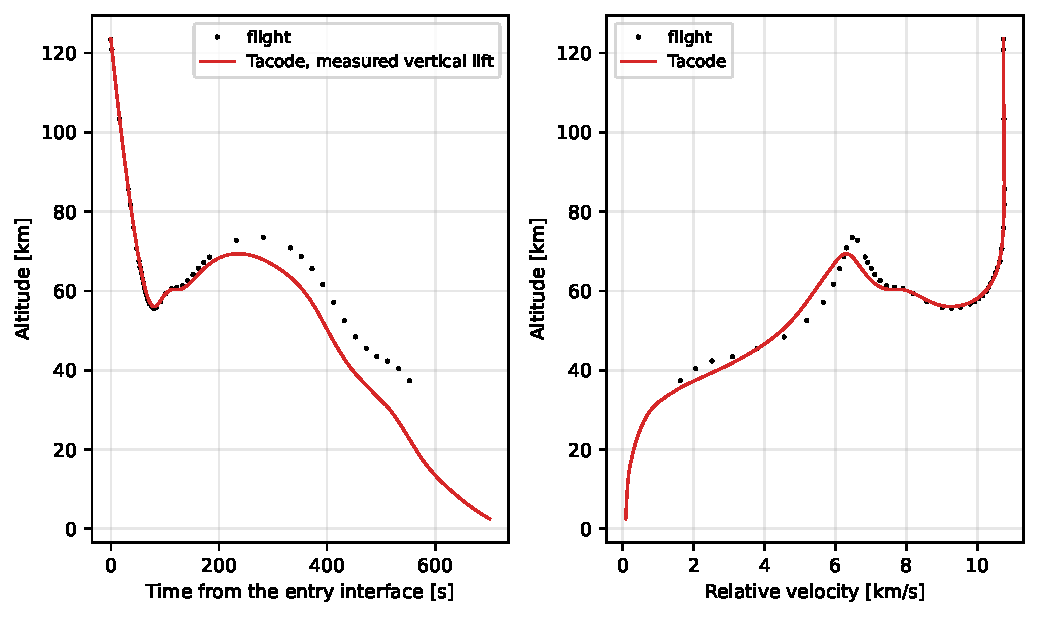
\includegraphics[width=0.95\linewidth]{apollo4_trajectory}
\end{center}
\caption{実測の鉛直揚力による Apollo 4: 突入界面からの時刻に対する高度（左）と
高度--速度平面（右）。}
\label{apollo4_trajectory}
\end{figure}

\subsection{Apollo 10}

Apollo 10 は\textbf{揚力について何も仮定しない}ケースである。NASA TN D-6725
\cite{Graves1972} は突入界面の状態ベクトル、誘導が実際に打ったロール角、そして実機が
飛んだ高度と速度を与える。ロール角\emph{が}揚力の向きなので、時刻に対する 89 節点の表
として入力に入り、高度と速度が比較対象になる。合わせ込む自由度は突入質量だけで、これは
参照文献に無い。

突入界面から 12〜414 s の 311 点に対し、高度は \textbf{3.2 km rms}（最大 $+5.5$ km）、
慣性速度は 189 m/s rms で一致する（図 \ref{apollo10_trajectory}）。この 3.2 km は
3 自由度の突入計算の誤差収支すべてである。大気テーブル、一定の係数、仮定した質量、
入力と参照の両方の読み取り、そして欠けている自由度が、まとめてこの中にある。

この数値を解釈可能にしているのは感度の掃引である。$C_L$ を $0.03$ 動かすと
——これは報告書自身が予測 $L/D$ の精度として挙げている値である——高度は基準誤差の 2〜3 倍
動く。つまり\textbf{制限しているのはソルバーではなく揚力係数}である。仮定した質量は
10 \% あたり約 1 km、時間刻みは何も効かない。揚力を切ると 33 km rms になり、これも
また精度ではなく欠落モデルの大きさである。

\begin{figure}[h]
\begin{center}
	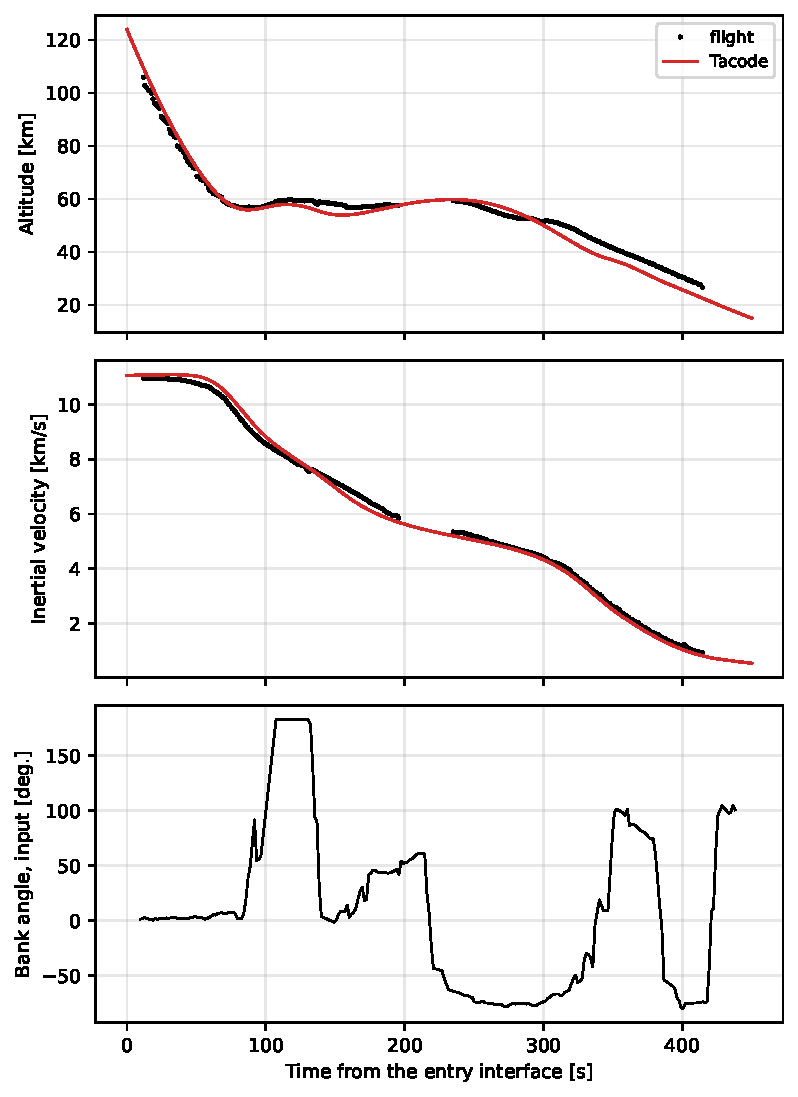
\includegraphics[width=0.55\linewidth]{apollo10_trajectory}
\end{center}
\caption{Apollo 10: 飛行に対する高度と慣性速度、およびこのケースを駆動する実測バンク角。}
\label{apollo10_trajectory}
\end{figure}

%----------------------------------------------------------------------
\subsection{Project Fire flight II} \label{fire2}

\subsubsection{なぜこの飛行か}

2 つの Apollo ケースは並進ソルバーを叩く。\emph{姿勢}ソルバーを実証するには姿勢の実測が
公表されている飛行が要るが、コード側の制約が候補を大きく絞る。Tacode には制御トルクが
無いので機体は無制御でなければならない。空力テーブルの軸は全迎角と Knudsen 数であって
Mach 数ではないので、係数が Mach に鈍い領域に留まる飛行でなければならない。そして
表化した空力は回転体を前提とするので、非対称が駆動する運動は表せない。

この 3 つで有力候補は落ちる。Apollo の突入と誘導のある突入機は第一の理由で、
ADEPT SR-1 と IRVE-3 は第二の理由で、公表された解析がまさに小さな質量・空力の非対称に
ついてである Reentry F は第三の理由で落ちる。Stardust は無制御・軸対称だったが姿勢が
測られていない。

Project Fire flight II はこの 3 つすべてを通る。月から帰還する鈍頭体の輻射加熱を調べる
ために 1965-05-22 に打ち上げられ、その再突入体は 171 rpm でスピン安定、完全に無制御、
軸対称であり、\textbf{3 軸のレートジャイロと 3 軸の加速度計}を積んでその記録が公表されて
いる \cite{Scallion1967}。11 351 m/s、経路角 $-14.7^\circ$ で突入した。

\subsubsection{資料が何であるか}

2 つの報告書を使う。それぞれの数値が表 \ref{validation_cases} のどの層かが重要である。

\begin{itemize}
\item \textbf{NASA TN D-3569 表 V} \cite{Lewis1966} が軌道で、0.5 秒刻み 625 点である。
その正式な題名は「再突入軌道パラメータ、\emph{計算機シミュレーションによる}」であり、
$t = 1608$ s のアセンション島レーダを初期条件とし、2 発の Nike-Apache 観測ロケットで
測った大気を飛ばした NASA 自身の 3 自由度質点計算である。すなわち層 B である。報告書は
これがブラックアウトの前後でレーダ軌跡と滑らかに繋がり、着水点を実測と 500 m 以内で
再現すると示している。良い参照ではあるが、これと合うことはソルバーの検証であって飛行の
物理の検証ではなく、抽出したデータファイル自身のヘッダにそう書いてある。
\item \textbf{NASA TN D-4183 図 4} \cite{Scallion1967} は迎角に対する静的係数 $C_X$、
$C_R$、$C_m$ で、Ames の極超音速自由飛行装置で Mach 35 で測ったものである。層 C、すなわち
入力である。これには有用な性質がある。報告書自身が飛行のレートジャイロ記録から迎角を出す
のにこの図を使っているので、\textbf{Tacode が飛ばす係数と「実測の迎角」の裏にある係数が
同じ数字になる}。
\item \textbf{NASA TN D-4183 図 17 と図 19} が姿勢の実測、層 A であり、
第 \ref{fire2_attitude} 節で扱う。
\end{itemize}

\subsubsection{何が確かめられるかを先に決める}

これは数値を 1 つも計算する前に書き下した。そうしないと、報告が「たまたま合った区間の
選択」になってしまうからである。

\emph{確かめられること}: 全 312 s の軌道、観測ロケット密度に対する大気テーブル、そして
ピッチ・ヨー振動の周期。

\emph{確かめられないこと}: 迎角包絡線の成長。その段はすべて Tacode が表せない離散的な
擾乱が作ったものである。スピンの減衰も同じ理由。そして Mach 3 以下のすべて。Tacode の
テーブルにも表 V にも Mach 軸が無いからである。

\subsubsection{データの読み取り}

表 V は数値表だが、1966 年の走査版でしか残っておらず、埋め込まれた文字認識が桁を落とし、
``E'' を ``EUR''、``.'' を ``-'' と読み、数を 1 文字ずつに砕いている。抽出は 1 つの原則で
書いた。\textbf{内挿で埋めない。}読めない値は \texttt{nan} と書いて数える。7761 個中
918 個がそれである。

\emph{復元できる}ものは証拠から復元する。動圧・気圧・密度の 3 列は SI と英単位で二度
印字されており、これは同じ数の独立した 2 回目の読み取りである。片方が壊れていればもう
片方から厳密に復元でき、両方生きていれば相互検証になる。近傍の中央値から桁ごと離れた値は
指数の脱落なので捨てる。近傍すべてが逆符号で、大きさは合っている値は、負号の脱落なので
復元する。

配置は文字の並び順ではなく座標から組み直す。行の間隔が開くと抽出ツールが 1 レコードを
列方向に歩くからである。\textbf{印字された 3 行のどれに属するかは、レコードごとに縦位置を
まとめて決める。固定しきい値では決めない。}走査が傾いているページがあり、そこでは同じ行の
右端の列が左端より行間隔の大部分だけ上に来る。しきい値で切ると密度が経路角の列に入る。
この不具合は、見つかるまでに密度と温度の列の 4 分の 1 を失わせていた。

表が満たすべき恒等式は診断として報告し、値の選別には\emph{使わない}。
$q_\infty = \rho V^2/2$ は中央値 $4 \times 10^{-7}$、$M = V/a$ は $5 \times 10^{-6}$、
$p = \rho R T$ は $2 \times 10^{-5}$ で成り立つ。ただし 95 km より上では組成が変わって
$R$ が 287.05 でなくなるため外れる。これは走査ではなく表そのものの性質である。

図 4 は 600 dpi で読み取った。較正は図自身の罫線で検査してあり、罫線は $C_X$ で 0.005、
$C_R$ で 0.002、$C_m$ で 0.0003 の精度で目盛りの値に乗る。\textbf{迎角軸の原点は枠の
左端ではない。}縦罫線は 16 本が $5^\circ$ ごとにあり、左端は $0$ ではなく $5^\circ$ である。
枠を原点と取ると全係数が $5^\circ$ ずれ、$C_D$ が 1.477 ではなく 1.467 になり、さらに悪い
ことに $C_m$ の微小迎角の傾きがほぼ 2 倍になる。この曲線の曲率のほとんどが最初の 5 度に
集まっているからである。この誤りは目ではなく物理で捕まえた。6 自由度計算の振動周波数が
解析解と食い違い、その食い違い方が $C_{m\alpha}$ を名指ししていた。直した較正では
$\alpha = 80^\circ$ が、文書の文字層にある ``80'' ラベルの位置と 1 画素で一致する。
読み取った係数を図 \ref{fire2_aerodynamics} に示す。

\begin{figure}[h]
\begin{center}
	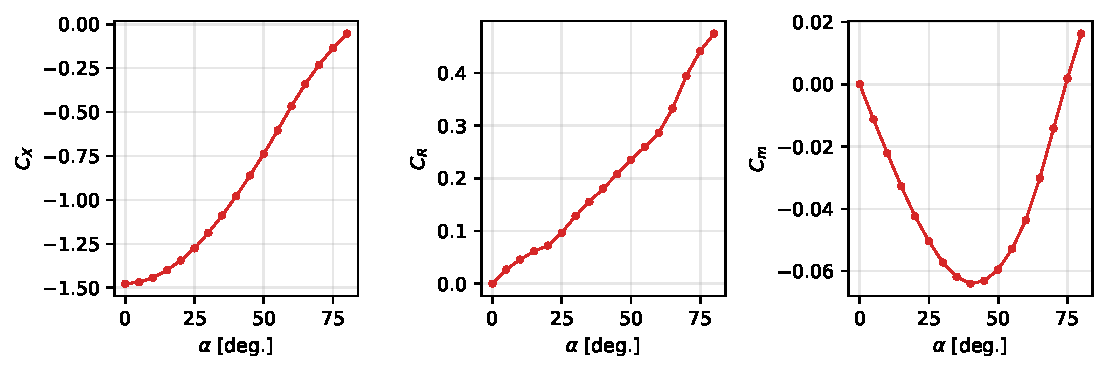
\includegraphics[width=0.98\linewidth]{fire2_aerodynamics}
\end{center}
\caption{Fire 再突入体の静的空力係数。NASA TN D-4183 図 4（Ames 極超音速自由飛行装置、
Mach 35）から読み取った。$C_D(0) = 1.4766$、図の基準点まわりで
$C_{m\alpha} = -0.129$ /rad。}
\label{fire2_aerodynamics}
\end{figure}

\subsubsection{機体と、その弾道係数が一定である理由}

再突入体は飛行中にベリリウム熱量計 3 枚とフェノール・アスベスト遮蔽 2 枚を順に捨て、
質量の 24 \%、ピッチ慣性の 34 \% を失う（表 \ref{fire2_mass}）。表 V を一読すると NASA が
これを無視したように見える。表 V は動圧と加速度の両方を印字しているので弾道係数を
$C_D S/m = -a g / q_\infty$ として逆算でき、それが使える 500 レコード全部で
$6.1490 \times 10^{-3}$ m$^2$/kg と 4 桁一致するからである。

無視したのではなく、そうならないように機体が作られていた。\textbf{質量と前面積を同じ割合で
捨てる}のである。5 つの構成にわたって弾道係数は $\pm 2.4$ \%、姿勢周波数を決める
$I_{yy}/d^3$ は $\pm 3.6$ \% しか動かない。表の時刻で質量・慣性・直径を階段状に変える
連鎖計算をしても、高度の一致は 126 m rms から 124 m rms へ動くだけである。
\emph{階段にしても変わらないこと}が結果であり、1966 年に一定の弾道係数を使ったのが妥当で
あった理由でもある。

\begin{table}[h]
\caption{Fire II 再突入体: NASA TN D-4183 表 I の 5 構成と、そこから導いた弾道係数と
慣性パラメータ。突入質量は TN D-3569 表 III の 86.568 kg を採る。TN D-4183 表 I は
86.586 と印字しているが、TN D-3569 表 I の積み上げは $94.73 - 8.16 = 86.57$ kg で終わり、
前者はこれに丸まるが後者は丸まらない。}
\label{fire2_mass}
\begin{center}
\begin{tabular}{l|r|r|r|r|r|r}
\hline \hline
構成 & $t$, s & 質量, kg & $d$, m & $I_{yy}$, kg m$^2$ & $m/(\pi d^2/4)$ & $I_{yy}/d^3$ \\
\hline
完全体                & 1617.75 & 86.568 & 0.672 & 2.806 & 244.1 & 9.25 \\
熱量計 1 枚目投棄     & 1640.48 & 83.189 & 0.651 & 2.644 & 249.9 & 9.58 \\
フェノール 1 枚目投棄 & 1642.12 & 76.022 & 0.630 & 2.305 & 243.9 & 9.22 \\
熱量計 2 枚目投棄     & 1646.10 & 72.166 & 0.607 & 2.128 & 249.4 & 9.52 \\
フェノール 2 枚目投棄 & 1647.53 & 66.179 & 0.587 & 1.857 & 244.5 & 9.18 \\
\hline \hline
\end{tabular}
\end{center}
\end{table}

Tacode は計算の途中で機体を変えられず、リスタート機能も未実装なので、連鎖はケース側で
駆動する。各区間を次の構成変化まで走らせ、その結果ファイルの最終状態を次の区間の初期
条件にする。必要な量はすべて、制御ファイルが要求する規約のまま出力に書かれている。
1 つ罠を記録しておく。\textbf{区間の計算は 1 ステップごとに出力させなければならない。}
そうしないと最後のレコードが区間の終わりより最大で出力間隔ぶん手前になり、ほぼ鉛直な
降下の 0.5 秒は 700 m になる。

\subsubsection{軌道}

突入状態は表 V の $t = 1618.25$ s から取る。121 920 m の突入界面の 0.5 秒後であり、
走査が最初のレコードの緯度・経度を落としているためである。表の地球相対の速度・経路角・
方位角を、地心ローカル水平系の ECEF 速度に変換して与える。

計算は 2 本行う。1 本目は Mach 35 で測った値 $C_D = 1.4766$ を飛ばす。2 本目は表 V 自身の
弾道係数が示す $C_D = 1.5009$ を飛ばし、\emph{入力}を同一にして、残るものがソルバーと
重力モデルと大気テーブルだけになるようにする。2 つの抗力係数の差は 1.6 \% である。
結果を表 \ref{fire2_trajectory_results} と図 \ref{fire2_trajectory} に示す。

\begin{table}[h]
\caption{Fire II: 走査が値を残しているレコードに対する、表 V との差。極超音速の窓は
$t = 1700$ s までで、それ以下では Tacode のテーブルにも表 V にも Mach 軸が無い。}
\label{fire2_trajectory_results}
\begin{center}
\footnotesize
\begin{tabular}{l|l|c|c|c}
\hline \hline
計算 & 区間 & 高度 & 相対速度 & 経路角 \\
\hline
$C_D = 1.4766$（図 4） & 全区間 & max $+231$ m, rms 126 m & rms 12.2 m/s & rms $0.16^\circ$ \\
                       & 極超音速 & max $-179$ m, rms 117 m & rms 23.1 m/s & rms $0.11^\circ$ \\
$C_D = 1.5009$（表 V） & 全区間 & max $+333$ m, rms 182 m & rms 13.0 m/s & rms $0.16^\circ$ \\
                       & 極超音速 & max $-79$ m, rms \textbf{48 m} & rms 25.0 m/s & rms \textbf{$0.09^\circ$} \\
区間ごとに質量を階段化 & 全区間 & max $+217$ m, rms 124 m & rms 12.0 m/s & rms $0.17^\circ$ \\
\hline \hline
\end{tabular}
\end{center}
\end{table}

\textbf{入力を同一にすると、Tacode は同じ突入に対する NASA の積分を、高度 48 m rms、
経路角 $0.09^\circ$ rms で再現する。}120 km から 20 km までの 82 秒、73 $g$ の減速ピークを
通してである。高度の $4 \times 10^{-4}$ にあたり、本稿の中で最も鋭いソルバー検証である。
図 4 の $C_D$ による 117 m はソルバーの誤差ではなく、2 つの抗力係数の 1.6 \% の差である。
どちらが正しいかは 1965 年の空力見積もりについての問いであってコードの問いではない。
Mach 3 以下では両者が数百 m 流れるが、これは Mach 依存の欠落である。時間刻みは何も寄与
しない。$\Delta t$ を 0.005 から 0.1 s まで動かしても高度 rms は 2 m しか動かない。

\begin{figure}[h]
\begin{center}
	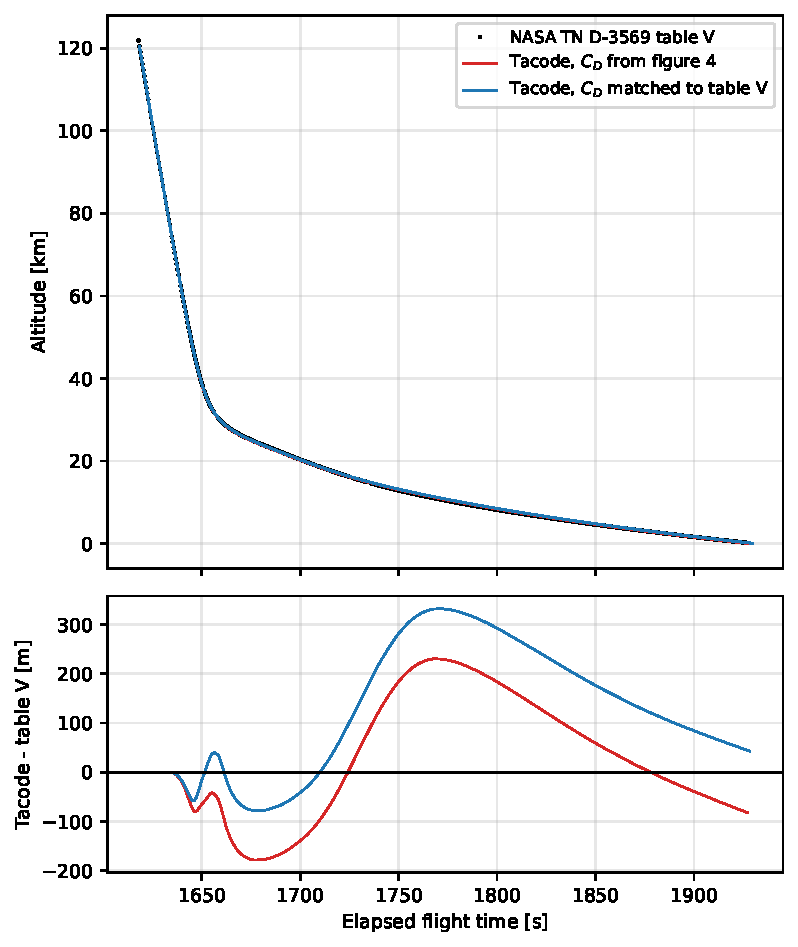
\includegraphics[width=0.58\linewidth]{fire2_trajectory}
\end{center}
\caption{Fire II の軌道と NASA TN D-3569 表 V、およびその残差。}
\label{fire2_trajectory}
\end{figure}

\subsubsection{大気}

表 V は軌道が飛んだ大気の密度・気圧・温度を持っており、これは 2 発の Nike-Apache 観測
ロケットによるもの、すなわち層 A である。これを Tacode が飛ぶ NRLMSISE-00 テーブルと
比べるのに軌道は関与しない（表 \ref{fire2_density_table}、図 \ref{fire2_density}）。
平均比は 0.994、rms のばらつきは 7.9 \% である。60 km 以下では 0.1 \% で一致するが、
これは勝利というより「どちらもそこでは標準大気に近い」という記述である。100〜122 km の
25 \% は熱圏で、太陽活動指数が効く。1965 年 5 月の太陽活動極小に対して $F_{10.7} = 75$ を
使った（当日の指数はオフラインで入手できなかった）。ただしそこでは動圧が 2 N/m$^2$ 以下で、
軌道は気にしない。

\begin{table}[h]
\caption{Fire II: NRLMSISE-00 テーブルと飛行で測られた密度。}
\label{fire2_density_table}
\begin{center}
\begin{tabular}{l|c|c|c|c|c|c|c}
\hline \hline
高度, km & 全体 & 0--20 & 20--40 & 40--60 & 60--80 & 80--100 & 100--122 \\
\hline
点数 & 535 & 392 & 91 & 15 & 11 & 12 & 14 \\
平均比 飛行/テーブル & \textbf{0.994} & 0.999 & 0.999 & 0.999 & 1.093 & 0.965 & 0.750 \\
\hline \hline
\end{tabular}
\end{center}
\end{table}

\begin{figure}[h]
\begin{center}
	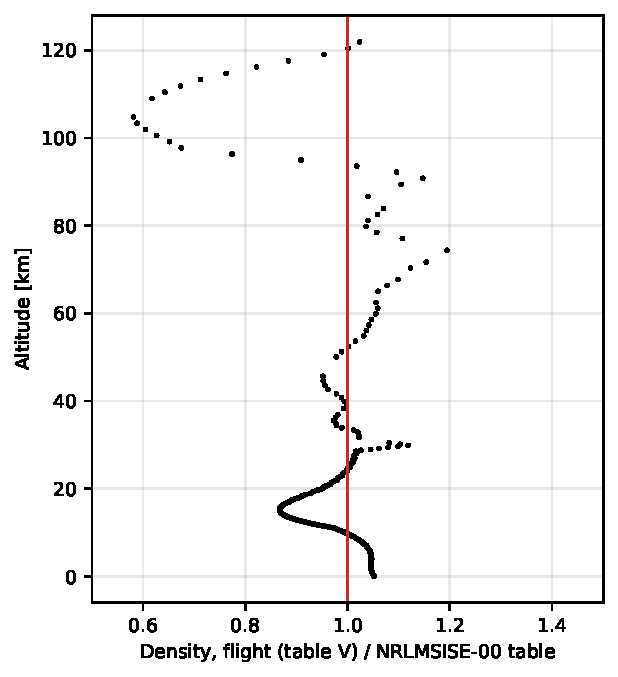
\includegraphics[width=0.42\linewidth]{fire2_density}
\end{center}
\caption{Fire II: Nike-Apache 観測ロケットが測った密度と、このケースが飛ぶ NRLMSISE-00
テーブルの比。}
\label{fire2_density}
\end{figure}

\subsubsection{姿勢} \label{fire2_attitude}

TN D-4183 の図 17 は 2 つを描いている。軌道の動圧（破線）と、\textbf{報告書自身の
6 自由度シミュレーションが実測のピッチ・ヨーレートの周波数に合わせるために必要とした
動圧}（実線、短い区間）である。彼らは風洞の $C_{m\alpha}$ を固定して動圧を振り、周波数を
合わせた。したがってその実線\emph{が}実測の周波数を動圧という単位で書いたものである。

これを周波数に直すには正しい関係式が要り、スピンする機体では式 (\ref{period}) ではない。
スピンする軸対称体の横方向運動は 2 つのモードに分かれ、tricyclic 解 \cite{Murphy1963} を
機体軸へ戻すと、遅いほうは
%
\begin{align}
	\lambda = p - a + \sqrt{a^2 + k \, q_{\infty}} ,
	\qquad
	a = \frac{I_{xx} \, p}{2 I_{yy}} ,
	\qquad
	k = - \frac{ C_{m\alpha} S d }{ I_{yy} }
	\label{tricyclic}
\end{align}
%
に現れる。動圧 0 では $\lambda = p$ になるが、これは「空間に固定された迎角を、回っている
機体から見れば毎秒 $p$ だけ回って見える」というだけの意味であり、無トルクの章動
（ここでは $(I_{xx} - I_{yy}) p / I_{yy} = 4.5$ rad/s）とは別のモードである。この 2 つを
取り違えると $C_{m\alpha}$ が倍近く違って出る。実際、本作業中に一度そうなった。

比較スクリプトは式 (\ref{tricyclic}) を\emph{仮定しない}。$k$ を Tacode の計算に当てはめ、
その形がどれだけ成り立つかを報告する。これ自体が検証になっている。

\begin{itemize}
\item この関係は計算の 75 個の窓に対し \textbf{0.05 rad/s rms} で当てはまる。周波数が
27〜46 rad/s なので 0.15 \% である。
\item 当てはめた $k$ が対応する $C_{m\alpha}$ は $-0.1418$ /rad である。読み取った表の
モーメントを図の基準点から重心へ移した値 $-0.1423$ に対して\textbf{0.4 \%}であり
（表そのものは $-0.1290$）、空力テーブル・重心移動・剛体ソルバーが互いに整合していることを
示す。
\end{itemize}

図 17 の 6 つのシミュレーション窓のうち 4 つは破線から綺麗に分離できる（残り 2 つは
破線の急な斜面に乗っている）。比較を表 \ref{fire2_frequency} と
図 \ref{fire2_attitude_figure} に示す。

\begin{table}[h]
\caption{Fire II: 振動周波数と実測との比較。一次量は動圧の比であり、周波数の列はそれを、
Tacode の計算に当てはめた $k$ で式 (\ref{tricyclic}) を通して写したものである。}
\label{fire2_frequency}
\begin{center}
\footnotesize
\begin{tabular}{c|r|r|c|r|r|c}
\hline \hline
窓, s & $q_\infty$ Tacode, N/m$^2$ & $q_\infty$ 要求, N/m$^2$ & 比 &
$\omega$ 計算, rad/s & $\omega$ 実測, rad/s & 比 \\
\hline
1644.9 &  66\,652 &  67\,569 & 1.014 & 37.17 & 37.35 & 1.005 \\
1649.3 & 117\,344 & 133\,438 & 1.137 & 45.93 & 48.33 & \textbf{1.052} \\
1652.6 & 108\,241 & 112\,185 & 1.036 & 44.51 & 45.13 & 1.014 \\
1662.4 &  26\,337 &  26\,156 & 0.993 & 27.74 & 27.69 & 0.998 \\
\hline \hline
\end{tabular}
\end{center}
\end{table}

\textbf{Tacode が予測する振動は、実機が飛んだ振動の 5 \% 以内にある。}4 つの窓の平均で
1.7 \%、最大の誤差は動圧のピークにある。区間を階段化した計算も 0.2 \% の違いで同じ答えを
与える。

この 5 \% は試験の分解能に近い。報告書は自分の図 17 の 2 本の差を「大気の測定と風洞
データ、あるいはその両方の不確かさ」に帰しており、その図の読み取り自体も 600 N/m$^2$ rms
の値打ちしかない。これは図の破線が表 V の動圧をどれだけ再現するかで測った値であり、
すなわち較正がどれだけ確かかを示している。

\begin{figure}[h]
\begin{center}
	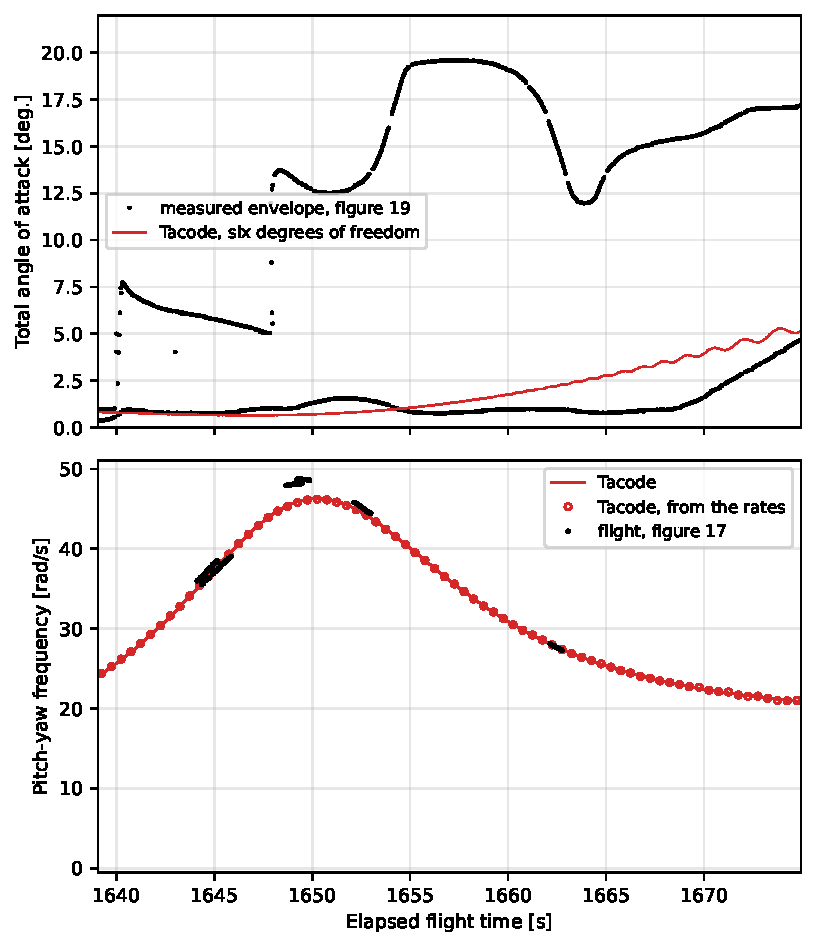
\includegraphics[width=0.58\linewidth]{fire2_attitude}
\end{center}
\caption{Fire II の姿勢。上: 全迎角と図 19 の実測包絡線。これらは比較\emph{できない}もの
であり、欠落の大きさを示すために並べて描いている。下: ピッチ・ヨー周波数。}
\label{fire2_attitude_figure}
\end{figure}

\subsubsection{意図的に比較しないもの}

図 19 の区間で、Tacode の全迎角は $0.64^\circ$ から $5.29^\circ$ の間に留まるが、実測の
包絡線は $0.36^\circ$ から $19.59^\circ$ まで登る。\textbf{これに誤差を付けないのは、
両者が比較にならないからである。}実測の包絡線は階段であり、段はすべて擾乱である。
$t = 1640.38$ s のベリリウム熱量計 1 枚目の非対称な溶融（角力積 6.440 N m s）、
1648.18 s のフェノール遮蔽 2 枚目の投棄（9.49 N m s）、そして 1652.7 s から始まる、
報告書自身が特定できなかった一連の事象である。Tacode にはそのどれも表す手立てが無い。

角力積を入れることは\emph{できた}。報告書は大きさを測っている。しかし向きは書いていない。
包絡線を再現した計算は、そうなるように向きを選んだものになる。それは合わせ込みであって
実証ではない。同じ理由で、連鎖計算は質量・慣性・直径だけを階段化し、スピンは一定に保って
いる。実機は $t = 1658$ から 1662 s の間に、これも報告書が説明できなかった擾乱で
スピンの半分を失っている。

報告書の図のうち 3 つは、検討したうえで意図的に読み取らなかった。スクリプトにその理由を
記録してある。TN D-4183 の図 8 はロールレートの標本のばらつきが大きく、報告書が本文に
数値を書いているから。図 9 は記号が重なりすぎており、200 個ほどのうち 30 個しか分離できず、
しかもその 30 個は疎な区間に偏るので標本が偏るから。TN D-3569 の図 17（レーダとの比較）は、
3 つの量と 4 種類の追尾装置が重なっていて読み取り精度が高度で約 1.5 km、測ろうとしている
一致の 10 倍粗いからである。

%----------------------------------------------------------------------
\section{計算例}

図 \ref{example_orbit} から図 \ref{example_reentry_6dof} は、コードに同梱している 3 つの
チュートリアルである。5000 s の低軌道、弾道再突入、そして同じ再突入を 6 自由度で解いた
ものである。これらは回帰ケースでもあるので、出力がコードとともに置いてあり、テストが
相対 $10^{-9}$ で再現を検査している。

\begin{figure}[h]
\begin{center}
	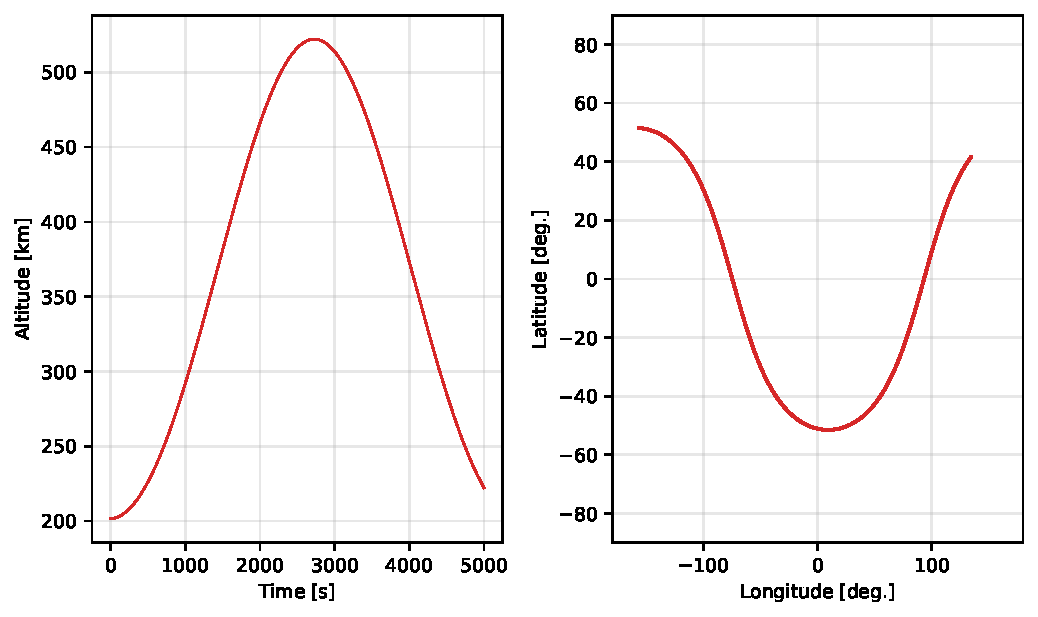
\includegraphics[width=0.85\linewidth]{example_orbit}
\end{center}
\caption{チュートリアル \texttt{work}: 5000 s の地球低軌道。時刻に対する高度（左）と
地上軌跡（右）。}
\label{example_orbit}
\end{figure}

\begin{figure}[h]
\begin{center}
	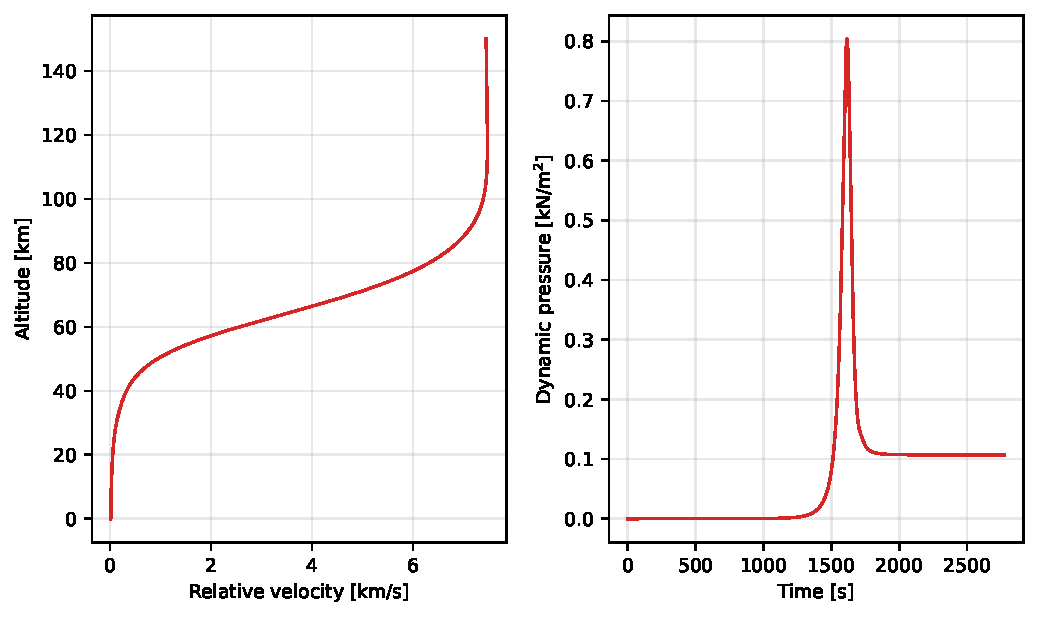
\includegraphics[width=0.85\linewidth]{example_reentry}
\end{center}
\caption{チュートリアル \texttt{work\_reentry}: 弾道再突入。高度--速度平面（左）と動圧（右）。}
\label{example_reentry}
\end{figure}

\begin{figure}[h]
\begin{center}
	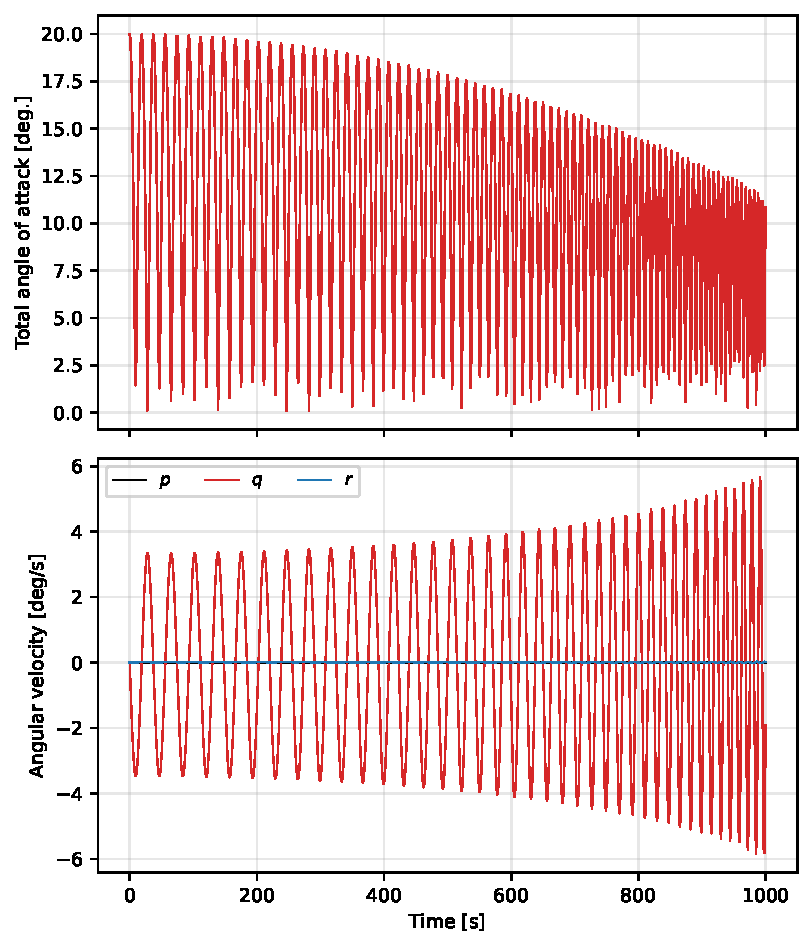
\includegraphics[width=0.55\linewidth]{example_reentry_6dof}
\end{center}
\caption{チュートリアル \texttt{work\_reentry\_6dof}: 同じ突入を姿勢込みで解いたもの。
全迎角（上）と ECEF に対する機体軸角速度（下）。式 (\ref{period}) のとおり、振動周波数は
動圧とともに上がる。}
\label{example_reentry_6dof}
\end{figure}

%----------------------------------------------------------------------
\section{まとめ}

Tacode version 2 は、version 1 の質点の定式化に、剛体の回転自由度、指定したバンク角で
向きを決める揚力、風、絶対時刻、そして発散の検知を足したものである。これらはすべて
既定で無効であり、無効なら出力はバイト単位で変わらない。回帰テストがそれを強制している。
この制約は偶然ではなく、意図した設計上の規則である。

正しさは 2 つの水準で示した。検証——厳密解・物理的な恒等式・変異テスト・バイト一致の
回帰に基づく 488 件の自動テスト——は方程式が書かれたとおりに解かれていることを示し、
73 $g$ の減速を含むケースでの積分器の実測収束次数は並進状態で 4.3、回転状態で 3.9 である。

3 つの飛行との突き合わせは、その方程式に何ほどの値打ちがあるかを示す。Apollo 4 と
Apollo 10 は、揚力の向きを飛行から取った揚力突入で並進ソルバーを叩く。良条件のほうである
Apollo 10 は 414 s の突入で高度 3.2 km rms で一致し、制限しているのはソルバーではなく
揚力係数である。Project Fire flight II は無制御スピン安定突入で、姿勢ソルバーを叩く。
同じ抗力係数のもとで軌道は NASA 自身の積分を 48 m rms で再現し、大気テーブルは観測
ロケットの密度と平均で 0.6 \% 一致し、\textbf{予測されたピッチ・ヨー振動は実機が飛んだ
ものの 5 \% 以内にある}。これは入手できる測定の分解能に近い。

結果の一部として同じだけ重要なのは、\emph{何を比較しないと決めたか}とその理由である。
Fire II の迎角包絡線の成長は、向きが公表されていない擾乱が駆動したものであること。
Apollo 4 の抗力のみの軌道の 27 km は精度ではなく欠落モデルの大きさであること。そして
3 つの図は、読み取り精度が測ろうとしている量より粗いこと。実証の報告は、自分の限界に
ついての説明の質を超えることはない。

%----------------------------------------------------------------------
\begin{thebibliography}{9}

\bibitem{Wagner1966}
C.~A. Wagner,
``The Gravity Potential and Force Field of the Earth Through Fourth Order'',
{\em NASA TN D-3317}, 1971.

\bibitem{Liu2019}
F.~Liu, S.~Lu and Y.~Sun,
{\em Guidance and Control Technology of Spacecraft on Elliptical Orbit},
Springer, 2019.

\bibitem{Lewis1966}
J.~H. Lewis, Jr. and W.~I. Scallion,
``Flight Parameters and Vehicle Performance for Project Fire Flight II, Launched
May 22, 1965'',
{\em NASA TN D-3569}, 1966.

\bibitem{Scallion1967}
W.~I. Scallion and J.~H. Lewis, Jr.,
``Body Motions and Angles of Attack During Project Fire Flight II Reentry'',
{\em NASA TN D-4183}, 1967.

\bibitem{Murphy1963}
C.~H. Murphy,
``Free Flight Motion of Symmetric Missiles'',
{\em Ballistic Research Laboratories Report No. 1216}, 1963.

\bibitem{Hillje1969}
E.~R. Hillje,
``Entry Aerodynamics at Lunar Return Conditions Obtained from the Flight of Apollo 4
(AS-501)'',
{\em NASA TN D-5399}, 1969.

\bibitem{Ried1972}
R.~C. Ried, Jr., W.~C. Rochelle and J.~D. Milhoan,
``Radiative Heating to the Apollo Command Module: Engineering Prediction and Flight
Measurement'',
{\em NASA TM X-58091}, 1972.

\bibitem{Graves1972}
C.~A. Graves, Jr. and J.~C. Harpold,
``Apollo Experience Report --- Mission Planning for Apollo Entry'',
{\em NASA TN D-6725}, 1972.

\end{thebibliography}

\end{document}
